\section{Results}
\label{sec:results}

Grand Slam results exploit the lottery for identification and are presented separately for the ATP and WTA tours. Non-Grand-Slam control-function results are summarized in Section~\ref{sec:results_nongs} and reported in full in the appendix.

\subsection{Immediate Effects}
\label{sec:results_immediate}

Table~\ref{tab:immediate} characterizes the treatment dose at the focal event. Because control players do not enter the main draw, these estimates describe the magnitude of the treatment rather than a causal effect against a counterfactual.

On the ATP tour ($N = 120$), treated players play additional main-draw matches and earn ranking points proportional to the round reached; the WTA pattern ($N = 82$) is similar. A Grand Slam first-round loss earns 10 ranking points and a second-round loss earns 45 points, so even a single main-draw win delivers an economically meaningful shock to the player's rolling 52-week ranking-point stock.

\begin{table}[htbp]
\centering
\caption{Grand Slam Lottery: Immediate Event-Level Effects}
\label{tab:immediate}
\begin{threeparttable}
\small
\begin{tabular}{l ccc}
\toprule
 & $t$-test & \multicolumn{2}{c}{Event FE} \\
\cmidrule(lr){2-2} \cmidrule(lr){3-4}
Outcome & LL Mean & $\hat{\beta}$ & (SE) \\
\midrule
\multicolumn{4}{l}{\textit{ATP}} \\
\quad Main-draw match win & 0.34$^{***}$ & 0.39$^{***}$ & (0.09) \\
\quad Main-draw matches played & 1.46$^{***}$ & 1.64$^{***}$ & (0.13) \\
\quad Ranking points at event & 28.85$^{***}$ & 36.35$^{***}$ & (5.50) \\
\quad $N$ & \multicolumn{1}{c}{61 / 59} & \multicolumn{2}{c}{120} \\
\addlinespace
\multicolumn{4}{l}{\textit{WTA}} \\
\quad Main-draw match win & 0.36$^{***}$ & 0.33$^{***}$ & (0.09) \\
\quad Main-draw matches played & 1.42$^{***}$ & 1.38$^{***}$ & (0.12) \\
\quad Ranking points at event & 25.45$^{***}$ & 23.93$^{***}$ & (4.35) \\
\quad $N$ & \multicolumn{1}{c}{33 / 49} & \multicolumn{2}{c}{82} \\
\addlinespace
\multicolumn{4}{l}{\textit{Pooled}} \\
\quad Main-draw match win & 0.35$^{***}$ & 0.38$^{***}$ & (0.06) \\
\quad Main-draw matches played & 1.45$^{***}$ & 1.53$^{***}$ & (0.09) \\
\quad Ranking points at event & 27.66$^{***}$ & 31.32$^{***}$ & (3.97) \\
\quad $N$ & \multicolumn{1}{c}{94 / 108} & \multicolumn{2}{c}{202} \\
\bottomrule
\end{tabular}

\begin{tablenotes}
\footnotesize
\item \textit{Notes.} First-time Grand Slam LL candidates: top-four ranked final-round qualifying losers at events with at least one LL slot, 2006--2024. ATP: $N = 120$; WTA: $N = 82$. Event FE columns report OLS with Grand Slam $\times$ Year fixed effects. Control outcomes are mechanically zero because unselected players do not enter the main draw. $^{***}p<0.01$, $^{**}p<0.05$, $^{*}p<0.10$.
\end{tablenotes}
\end{threeparttable}
\end{table}

\subsection{Post-Episode Dynamics}
\label{sec:results_dynamics}

Tables~\ref{tab:dynamic_atp} and~\ref{tab:dynamic_wta} report estimates from a stacked specification with horizon-specific treatment effects estimated jointly. The stacked model pools all five horizons into a single regression with horizon-specific LL coefficients and horizon fixed effects, improving efficiency by borrowing information across horizons while allowing the treatment effect to vary freely at each horizon.

On the ATP side, the sample comprises 120 first-time player-episodes contributing approximately 600 stacked observations across five horizons. The lottery raises ranking points by 72.5 at 4 weeks, 72.1 at 8 weeks, and 82.8 at 12 weeks (each significant at conventional levels), before peaking and starting to fade: the effect is 72.6 at 26 weeks (clustered $p = 0.047$; Fisher $p = 0.164$) and becomes indistinguishable from zero at 52 weeks. The 4-, 8-, and 12-week estimates survive Fisher randomization inference ($p_{Fisher} < 0.001$, $p_{Fisher} = 0.002$, $p_{Fisher} = 0.028$), so at those horizons the finding does not rely on the asymptotic approximation. The 26-week estimate does not survive Fisher inference and is the horizon at which small-sample noise begins to bite; it is the least robust of the significant effects. Benjamini-Hochberg $q$-values across the 80-test family of primary outcomes are reported in Appendix Table~\ref{tab:bh}: the ATP GS 4-, 8-, and 12-week ranking-point effects survive joint BH correction at $q < 0.05$; the 26-week effect does not ($q = 0.119$), and 23 of the 80 tests survive overall. Elo rating changes are null at every horizon, so the ranking-point gains come from more matches and rounds played rather than from measured ability improvement. The trajectory is consistent with the initial point shock being real but temporary: it accumulates through 12--26 weeks as the ranking boost opens further tournaments, then dissipates as the original points age out of the rolling window.

On the WTA side, the 82-episode sample delivers approximately 410 stacked observations. Ranking points rise by 55.0 at 8 weeks ($p = 0.017$); estimates at other horizons are positive but imprecise. The Elo pattern differs from the ATP tour: WTA first-timers show Elo gains at 8 weeks ($+15.0$, $p = 0.082$) and at 52 weeks ($+36.8$, $p = 0.055$). These estimates should be read against the borderline joint balance ($p = 0.063$) and the smaller sample. The Elo channel on the WTA is explored further in Section~\ref{sec:mechanisms}.

\begin{table}[htbp]
\centering
\caption{ATP Grand Slam: Post-Episode Dynamic Effects (Stacked Model)}
\label{tab:dynamic_atp}
\begin{threeparttable}
\small
\begin{tabular}{l*{5}{c}}
\toprule
 & 4w & 8w & 12w & 26w & 52w \\
\midrule
Ranking Pts $\Delta$ & 72.5$^{***}$ & 72.1$^{***}$ & 82.8$^{***}$ & 72.6$^{**}$ & 23.5 \\
 & (26.7) & (26.6) & (26.1) & (36.2) & (59.1) \\[0.3em]
Elo $\Delta$ & -4.4 & 0.2 & -4.8 & 4.7 & -9.7 \\
 & (9.1) & (10.9) & (10.3) & (13.5) & (21.0) \\[0.3em]
Main Draws & -0.2 & 0.1 & 0.1 & 0.7 & 0.8 \\
 & (0.5) & (0.5) & (0.5) & (0.5) & (1.5) \\[0.3em]
Matches 250+ & 0.3 & 0.7 & 0.9 & 1.5 & 1.3 \\
 & (1.0) & (1.0) & (0.9) & (1.1) & (2.8) \\[0.3em]
Win \% & 0.04 & -0.01 & -0.03 & -0.03 & -0.03 \\
 & (0.05) & (0.03) & (0.03) & (0.03) & (0.03) \\[0.3em]
\bottomrule
\end{tabular}

\begin{tablenotes}
\footnotesize
\item \textit{Notes.} Stacked specification: 120 first-time player-episodes contributing approximately 600 stacked observations across five horizons (4, 8, 12, 26, 52 weeks). Horizon-specific LL treatment effects estimated jointly with horizon fixed effects, Grand Slam $\times$ Year fixed effects, and pre-treatment controls (ranking points linear and quadratic, Elo / 100 linear and quadratic, surface Elo / 100 linear and quadratic, and age). Standard errors clustered at the player level. $^{***}p<0.01$, $^{**}p<0.05$, $^{*}p<0.10$.
\end{tablenotes}
\end{threeparttable}
\end{table}

\begin{table}[htbp]
\centering
\caption{WTA Grand Slam: Post-Episode Dynamic Effects (Stacked Model)}
\label{tab:dynamic_wta}
\begin{threeparttable}
\small
\begin{tabular}{l*{5}{c}}
\toprule
 & 4w & 8w & 12w & 26w & 52w \\
\midrule
Ranking Pts $\Delta$ & 40.0 & 55.0$^{**}$ & 27.8 & 7.5 & 26.5 \\
 & (28.5) & (22.5) & (20.1) & (42.8) & (86.4) \\[0.3em]
Elo $\Delta$ & 13.3$^{*}$ & 15.0$^{*}$ & 11.8 & 21.6$^{*}$ & 36.8$^{*}$ \\
 & (7.6) & (8.5) & (9.1) & (12.7) & (18.9) \\[0.3em]
Main Draws & -0.1 & 0.3 & 0.3 & 0.7 & 1.8 \\
 & (0.5) & (0.5) & (0.6) & (0.7) & (1.5) \\[0.3em]
Matches 250+ & -0.5 & 0.8 & 0.6 & 1.9$^{*}$ & 3.2 \\
 & (1.0) & (0.7) & (0.8) & (1.0) & (2.5) \\[0.3em]
Win \% & 0.03 & 0.05$^{*}$ & 0.05$^{*}$ & 0.04 & 0.05 \\
 & (0.05) & (0.03) & (0.03) & (0.03) & (0.03) \\[0.3em]
\bottomrule
\end{tabular}

\begin{tablenotes}
\footnotesize
\item \textit{Notes.} Stacked specification: 82 first-time player-episodes contributing approximately 410 stacked observations across five horizons (4, 8, 12, 26, 52 weeks). Horizon-specific LL treatment effects estimated jointly with horizon fixed effects, Grand Slam $\times$ Year fixed effects, and pre-treatment controls. Standard errors clustered at the player level. $^{***}p<0.01$, $^{**}p<0.05$, $^{*}p<0.10$.
\end{tablenotes}
\end{threeparttable}
\end{table}

Figures~\ref{fig:event_study_atp} and~\ref{fig:event_study_wta} plot mean cumulative ranking points earned by LL-selected and unselected players from 12 weeks before to 52 weeks after each Grand Slam. Pre-event trajectories on both tours are parallel, so pre-treatment divergence is not detectable. After the event, ATP LL recipients accumulate approximately 72 additional ranking points by 4 weeks and 83 by 12 weeks; the advantage then narrows as the rolling window absorbs the initial gains. WTA LL recipients diverge at 8 weeks by 55 points, with controls catching up more quickly than on the ATP tour, a pattern consistent with the denser WTA calendar.

\begin{figure}[htbp]
\centering
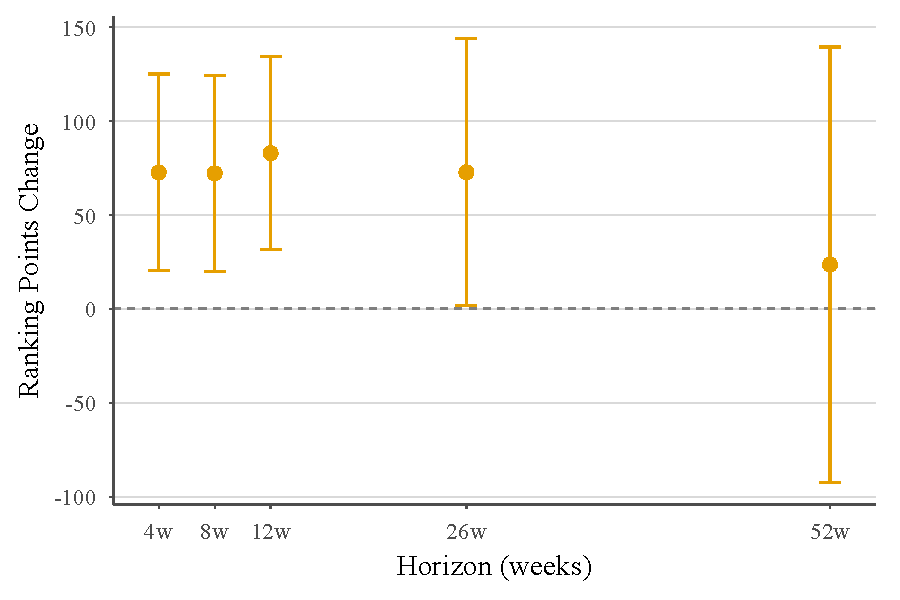
\includegraphics[width=0.85\textwidth]{../Figures_FirstLL/fig_event_study_atp.pdf}
\caption{ATP Event Study: Ranking Trajectories for Selected and Unselected Players}
\label{fig:event_study_atp}
\begin{minipage}{0.9\textwidth}
\vspace{0.5em}
\footnotesize \textit{Notes.} Each point is the estimated treatment effect at the indicated horizon. Vertical dashed line marks the event date. Shaded regions are 95 percent confidence intervals. First-time ATP Grand Slam sample ($N = 120$).
\end{minipage}
\end{figure}

\begin{figure}[htbp]
\centering
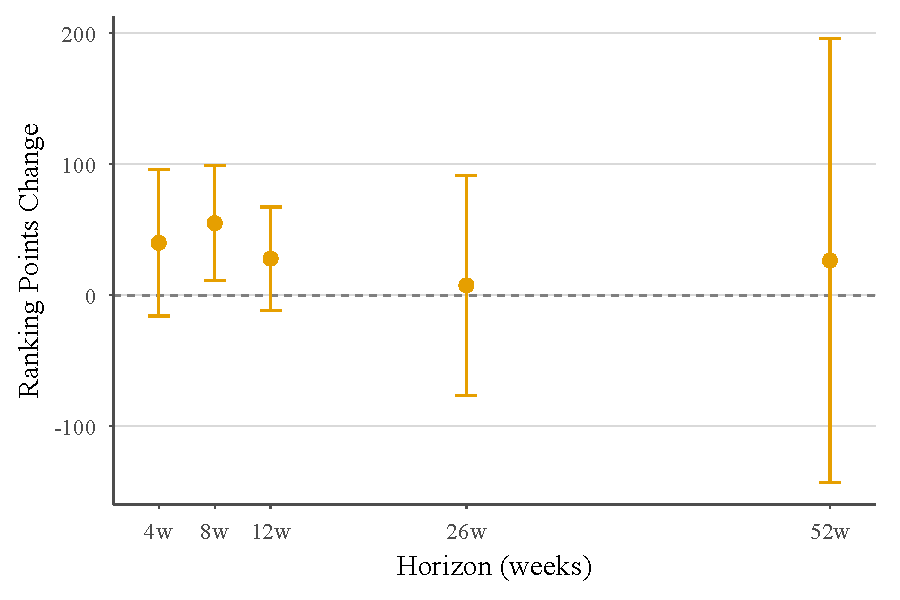
\includegraphics[width=0.85\textwidth]{../Figures_FirstLL/fig_event_study_wta.pdf}
\caption{WTA Event Study: Ranking Trajectories for Selected and Unselected Players}
\label{fig:event_study_wta}
\begin{minipage}{0.9\textwidth}
\vspace{0.5em}
\footnotesize \textit{Notes.} Each point is the estimated treatment effect at the indicated horizon. First-time WTA Grand Slam sample ($N = 82$).
\end{minipage}
\end{figure}

\subsection{Heterogeneous Effects}
\label{sec:results_heterogeneity}

The first-time GS sample is small ($N = 120$ ATP, $N = 82$ WTA), limiting statistical power for subgroup analysis. Table~\ref{tab:hetero_atp} reports heterogeneity for the ATP GS sample. Effects are stronger and more persistent for older players (age $\geq 24$): ranking-point gains of 154.9 at 26 weeks ($p < 0.001$) and 186.4 at 52 weeks ($p < 0.01$). This pattern is consistent with older players at the qualifying margin having more tournament experience to convert a ranking boost into sustained access, even with a shorter remaining career runway. Other subgroup contrasts, by pre-episode ranking and by surface, are imprecisely estimated in the small ATP sample.

The non-GS samples provide substantially more power for heterogeneity analysis ($N = 2{,}054$ ATP, $N = 1{,}423$ WTA); results are reported in Appendix Tables~\ref{tab:hetero_nongs_atp} and~\ref{tab:hetero_nongs_wta}.

\begin{table}[htbp]
\centering
\caption{ATP Grand Slam: Heterogeneous Effects}
\label{tab:hetero_atp}
\begin{threeparttable}
\small
\begin{tabular}{l*{5}{c}}
\toprule
 & 4w & 8w & 12w & 26w & 52w \\
\midrule
\multicolumn{6}{l}{\textit{Rank}} \\
  Ranking Pts $\Delta$ & 71.5$^{**}$ & 76.5$^{**}$ & 91.4$^{***}$ & 79.6$^{*}$ & 26.1 \\
  & (33.5) & (30.7) & (28.1) & (44.5) & (75.4) \\
  $\times$ High & 0.6 & -10.3 & -18.7 & -15.6 & -6.1 \\
  & (42.9) & (39.7) & (39.8) & (47.1) & (73.4) \\[0.3em]
  Main Draws & -0.7 & -0.4 & -0.2 & 0.8 & 1.3 \\
  & (0.6) & (0.6) & (0.6) & (0.6) & (1.7) \\
  $\times$ High & 1.2 & 0.9 & 0.8 & -0.3 & -1.0 \\
  & (0.8) & (0.8) & (0.8) & (0.9) & (2.1) \\[0.3em]
  Elo $\Delta$ & -8.8 & 0.6 & -4.3 & 22.3 & -3.7 \\
  & (9.5) & (10.5) & (10.7) & (16.5) & (25.0) \\
  $\times$ High & 8.1 & -1.4 & -1.5 & -34.7$^{*}$ & -12.2 \\
  & (14.5) & (15.2) & (16.2) & (19.1) & (25.9) \\[0.3em]
\midrule
\multicolumn{6}{l}{\textit{Age}} \\
  Ranking Pts $\Delta$ & 76.1$^{**}$ & 56.6 & 71.6$^{**}$ & 6.1 & -49.0 \\
  & (32.8) & (34.3) & (33.8) & (40.2) & (68.3) \\
  $\times$ High & -9.9 & 35.8 & 27.8 & 154.9$^{***}$ & 186.4$^{**}$ \\
  & (37.3) & (38.4) & (39.2) & (47.2) & (74.3) \\[0.3em]
  Main Draws & -0.2 & -0.3 & -0.3 & -0.4 & -1.3 \\
  & (0.6) & (0.6) & (0.6) & (0.6) & (1.7) \\
  $\times$ High & 0.1 & 0.9 & 1.1$^{*}$ & 2.5$^{***}$ & 5.2$^{**}$ \\
  & (0.7) & (0.7) & (0.6) & (0.8) & (2.1) \\[0.3em]
  Elo $\Delta$ & -9.7 & -7.1 & -14.7 & -13.6 & -19.5 \\
  & (11.5) & (13.0) & (12.9) & (15.4) & (24.1) \\
  $\times$ High & 13.9 & 18.6 & 24.5 & 45.7$^{**}$ & 23.7 \\
  & (15.2) & (15.7) & (17.3) & (19.2) & (25.5) \\[0.3em]
\midrule
\bottomrule
\end{tabular}

\begin{tablenotes}
\footnotesize
\item \textit{Notes.} Stacked specification with horizon-specific LL treatment effects estimated by subgroup. First-time ATP Grand Slam sample ($N = 120$), 2006--2024. Low/High rank points split at the tour-specific median. Younger/Older split at age 24. Standard errors clustered at the player level. $^{***}p<0.01$, $^{**}p<0.05$, $^{*}p<0.10$.
\end{tablenotes}
\end{threeparttable}
\end{table}

\subsection{Non-Grand-Slam Extension}
\label{sec:results_nongs}

The non-Grand-Slam control-function estimates provide corroborating evidence from substantially larger samples. On the ATP tour ($N = 2{,}054$), ranking-point gains are 20.6 at 4 weeks ($p = 0.041$) and 44.6 at 26 weeks ($p = 0.002$). Elo effects emerge at medium horizons: $+12.8$ at 8 weeks ($p = 0.018$) and $+30.8$ at 26 weeks ($p = 0.016$), a pattern that differs from the GS null and may reflect either the larger sample's power to detect moderate ability effects or a difference in the non-GS competitive environment.

On the WTA tour ($N = 1{,}423$), ranking-point gains are 23.2 at 12 weeks ($p = 0.057$), with Elo gains of 10.5 at 12 weeks ($p = 0.011$). The WTA non-GS Elo finding parallels the marginal WTA GS Elo result and points toward genuine, if modest, ability gains, plausibly linked to greater competitive parity on the women's tour.

The non-GS estimates align with the GS lottery estimates in both direction and magnitude, supporting the validity of the control-function approach. Full non-Grand-Slam dynamic tables are reported in Appendix Tables~\ref{tab:dynamic_nongs_atp} and~\ref{tab:dynamic_nongs_wta}; heterogeneity results are in Appendix Tables~\ref{tab:hetero_nongs_atp} and~\ref{tab:hetero_nongs_wta}.

The dose-response analysis examines whether treatment effects vary with the number of main-draw matches won at the focal event. The initial LL slot provides a ranking-point benefit that is amplified when the player wins matches in the main draw. Dose-response results are reported in the appendix.
